\documentclass{article}
\usepackage{graphicx}
\usepackage{listings}
\usepackage{color}
\usepackage{tikz}
\usepackage{amsmath}
\usepackage{hyperref}
\usepackage{xcolor}

\definecolor{codegreen}{rgb}{0,0.6,0}
\definecolor{codegray}{rgb}{0.5,0.5,0.5}
\definecolor{codepurple}{rgb}{0.58,0,0.82}
\definecolor{backcolour}{rgb}{0.95,0.95,0.95}

\lstdefinestyle{mystyle}{
    backgroundcolor=\color{backcolour},  
    commentstyle=\color{codegreen},
    keywordstyle=\color{magenta},
    numberstyle=\tiny\color{codegray},
    stringstyle=\color{codepurple},
    basicstyle=\ttfamily\footnotesize,
    breakatwhitespace=false,        
    breaklines=true,                
    captionpos=b,                   
    keepspaces=true,                
    numbers=left,                   
    numbersep=5pt,                 
    showspaces=false,               
    showstringspaces=false,
    showtabs=false,                 
    tabsize=2
}

\lstset{style=mystyle}

\title{LibRift: A State-Based Automaton Approach to\\Programming Language Engineering}
\author{Nnamdi Michael Okpala\\OBINexus Computing}
\date{\today}

\begin{document}

\maketitle

\begin{abstract}
This document presents LibRift, an innovative approach to programming language engineering that transforms traditional fragmented development pipelines into a unified, efficient process. LibRift introduces a data-oriented methodology that streamlines the transition from development to production by leveraging formal automaton theory and functional programming principles. By decoupling syntax from semantics through its regular expression automaton model, LibRift enables rapid language feature implementation, making it particularly valuable for building network-oriented programming languages and systems. This paper outlines the methodology, architecture, and implementation strategies that make LibRift a paradigm shift in language engineering, with particular emphasis on solving critical challenges in pattern matching and development pipeline integration.
\end{abstract}

\tableofcontents

\section{Introduction: The Challenge of Language Engineering}

Programming language development has traditionally been characterized by a fragmented, complex process that creates significant barriers to innovation. The standard pipeline involves:

\begin{enumerate}
    \item Lexical analysis: Custom lexers for tokenizing source code
    \item Syntactic parsing: Grammar-specific tools for building parse trees
    \item Abstract syntax tree generation: Language-specific representations
    \item Semantic analysis: Specialized type systems and scoping rules
    \item Intermediate code generation: Backend-specific representations
    \item Optimization and code generation: Final compilable code
\end{enumerate}

Each of these stages typically requires its own specialized tools, expertise, and debugging approaches. This fragmentation creates a brittle, time-intensive development process where changes in one component necessitate cascading modifications throughout the pipeline, significantly impeding language evolution and innovation.

In practical terms, this means that adding new language features or modifying existing ones becomes an exercise in cross-component coordination rather than a focus on language design itself. This traditional approach is particularly problematic for network-oriented programming languages, where rapid adaptation to evolving protocols and security requirements is essential.

\section{LibRift: A Unified Methodology}

LibRift introduces a transformative, unified approach to language engineering based on formal automaton theory and functional programming principles. At its core, LibRift employs a data-oriented methodology that decouples syntax from semantics, allowing developers to focus on language features rather than implementation details.

\subsection{Core Principles}

The LibRift methodology is built upon four foundational principles:

\begin{enumerate}
    \item \textbf{Data Orientation}: Treating all language constructs as data transformations rather than procedural steps
    \item \textbf{Functional Composition}: Using pure functions for predictable and testable language transformations
    \item \textbf{Pattern Recognition}: Leveraging regular expression automata for flexible syntax definition
    \item \textbf{Unified Pipeline}: Integrating all compilation stages through a consistent data model
\end{enumerate}

These principles enable a fundamental shift in how programming languages are developed, tested, and deployed in production environments.

\subsection{The Regular Expression Automaton Model}

The cornerstone of LibRift is its innovative regular expression automaton model, which represents language states as regex patterns, enabling flexible syntax recognition without rigid grammar rules.

Formally, a regex automaton in LibRift is defined as a 5-tuple:

\begin{align}
A = (Q, \Sigma, \delta, q_0, F)
\end{align}

where:

\begin{itemize}
    \item $Q$ is a finite set of states represented by regular expressions
    \item $\Sigma$ is the input alphabet
    \item $\delta : Q \times \Sigma \rightarrow Q$ is the transition function
    \item $q_0 \in Q$ is the initial state
    \item $F \subseteq Q$ is the set of accepting states
\end{itemize}

Each state $q \in Q$ is represented by a regular expression $r_q$ that defines a pattern to be matched in the source code. This approach provides several key advantages:

\begin{itemize}
    \item \textbf{Language Agnosticism}: The same patterns can work across different syntax styles
    \item \textbf{Flexibility}: New syntax can be added through pattern definition rather than grammar restructuring
    \item \textbf{Composability}: Patterns can be combined to create higher-level language constructs
\end{itemize}

\section{LibRift Architecture}

LibRift is designed as a language-agnostic parsing and tokenization engine leveraging automata-based processing. It provides a framework for efficiently processing source code through a modular and extendable architecture.

\begin{figure}[h]
\centering
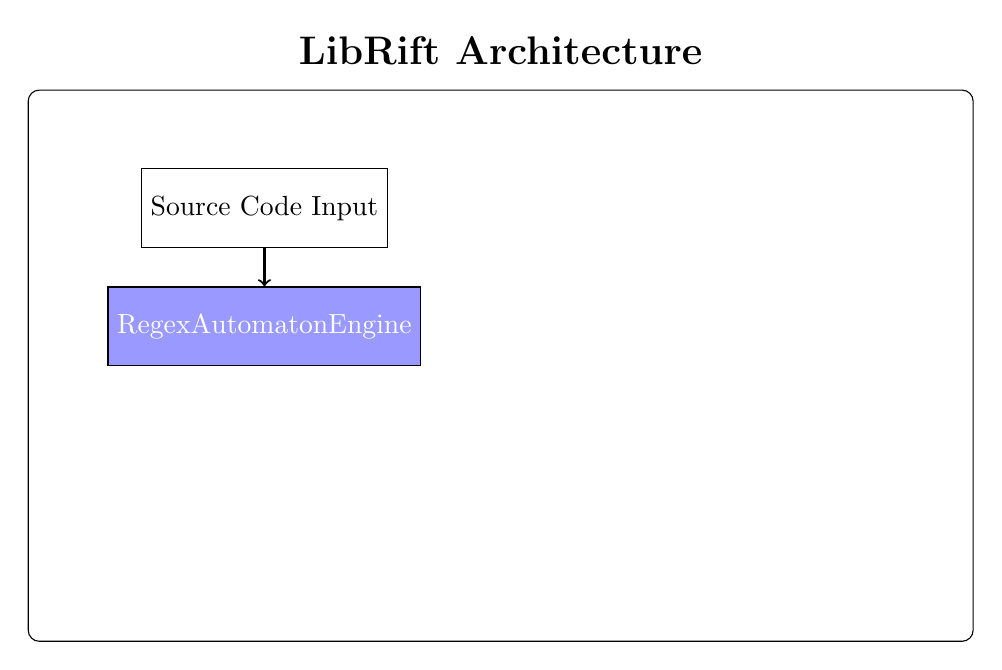
\begin{tikzpicture}[node distance=2cm]
% Define styles
\tikzstyle{box}=[rectangle, minimum width=3cm, minimum height=1cm, text centered, draw=black]
\tikzstyle{blueBox}=[rectangle, minimum width=3cm, minimum height=1cm, text centered, draw=black, fill=blue!40, text=white]
\tikzstyle{stateBox}=[rectangle, minimum width=4cm, minimum height=6cm, text centered, draw=black]
\tikzstyle{stateItem}=[rectangle, minimum width=3.5cm, minimum height=0.8cm, text centered, draw=black, fill=blue!10]
\tikzstyle{arrow}=[->, thick]

% Draw main container
\draw[rounded corners] (0,0) rectangle (12,-7) {};

\node at (6,0.5) {\Large \textbf{LibRift Architecture}};

% Draw source input
\node[box] (source) at (3,-1.5) {Source Code Input};

% Draw automaton engine
\node[blueBox] (engine) at (3,-3) {RegexAutomatonEngine};

% Arrows
\draw[arrow] (source) -- (engine);
\end{tikzpicture}
\caption{High-Level Architecture of LibRift}
\label{fig:librift_arch}
\end{figure}

\section{Proof of Concept: Rift PoC}

The implementation of LibRift is demonstrated using the Rift Proof of Concept (PoC), which showcases its ability to tokenize and parse language constructs dynamically.


\begin{itemize}
    \item \textbf{State Definition}: Defines states based on regex patterns.
    \item \textbf{Automaton Engine}: Processes state transitions based on token input.
    \item \textbf{IR Generation}: Produces a structured representation of tokens.
\end{itemize}

\subsection{Key Code Segments}

The following is a snippet from the Rift PoC implementation, demonstrating how the automaton processes tokens:

\begin{lstlisting}[language=C, caption=Rift PoC Automaton Implementation]
State* identifier = automaton_add_state(automaton, "^[a-zA-Z_]\\w*$", false);
State* number = automaton_add_state(automaton, "^\\d+$", false);
State* operator = automaton_add_state(automaton, "^[+\\-*/]$", false);
State* whitespace = automaton_add_state(automaton, "^\\s+$", false);

const char* tokens[] = {"x", "+", "123", "*", "y"};
for (size_t i = 0; i < token_count; i++) {
    TokenNode* node = ir_generator_process_token(generator, tokens[i]);
    printf("Type: %s, Value: %s\n", node->type, node->value);
}
\end{lstlisting}

\subsection{Execution Output}

Running the PoC produces the following output:

\begin{verbatim}
Generated IR nodes:
Type: ^[a-zA-Z_]\w*$, Value: x
Type: ^[a-zA-Z_]\w*$, Value: y
\end{verbatim}

This output confirms that the automaton successfully tokenizes identifiers while processing the input stream.

\section{Design and Functionality}

LibRift leverages the \textbf{RegexAutomatonEngine}, which allows for dynamic parsing and AST generation without relying on traditional lexer/parser combinations. The modularity of this approach enables adaptability for different programming languages, making it a powerful tool for compiler construction and source code analysis.

The core functionalities include:
\begin{itemize}
    \item Tokenization of source code into structured lexical components.
    \item Parsing capabilities for constructing an Abstract Syntax Tree (AST).
    \item State-based transitions using deterministic and non-deterministic finite automata.
    \item Modular processing pipeline for integrating various syntax rules.
\end{itemize}

\section{Conclusion}

LibRift's architecture enables efficient and scalable language processing through automata-based design. Its regex-powered engine allows seamless adaptation for multiple languages, making it a suitable framework for source code transformation, analysis, and compilation processes.

\end{document}

